\documentclass[]{article}

\usepackage[utf8]{inputenc}
\usepackage{array}
\usepackage{wrapfig}
\usepackage{multirow}
\usepackage{tabu}
\usepackage{graphicx}
\usepackage{amsmath,mathtools,amssymb}
\newcommand{\code}[1]{\texttt{#1}}
\usepackage{subfigure}

\usepackage{geometry}
 \geometry{
letterpaper,
 total={215mm,279mm},
 left=45mm,
 right=45mm,
 top=25mm,
tmargin = 15mm,
 bottom=25mm,
 }


\begin{document}

\title{Homework 1}
\author{Joshua Michalenko\\ ELEC 677: Deep Learning \\  Dr.\,Ankit Patel}
\date{10/04/16}
\maketitle



\section{Problem 1: Backpropogation in a simple Nueral Network}
\subsection{Part A:  Dataset}
The plot of the Two Moons dataset is displayed in Figure \ref{fig:partA}

\begin{figure}[ht]
        \centering
        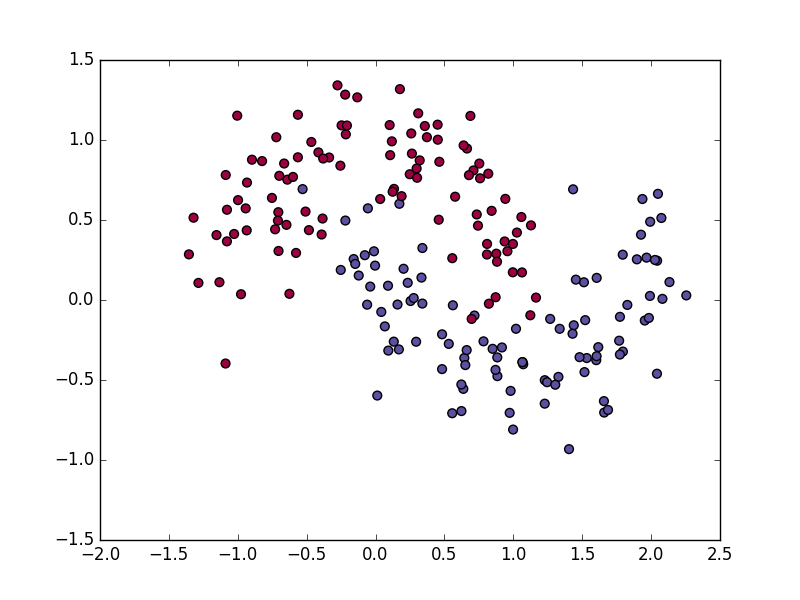
\includegraphics[width=10cm]{figures/twoMoons.png}

 	\caption{Two moons dataset displayed in matplotlib}

 	 \label{fig:partA}
\end{figure}


\subsection{Part B - Activation Functions}
\subsubsection{Part B1 - Implement activation functions}
If you look in my code you can see I implemented the activations function. 


\subsubsection{Part B2 - Derivative Derivations}
\paragraph{ Part B2.1 -  Derivative for Sigmoid function}

\begin{align*} 
\sigma(z)= f(z) = \frac{1}{1+e^{-z}}  &= (1+ e^{-z})^{-1} \\
\frac{df}{dz} : = -1* (1+ e^{-z})^{-2} * -e^{-z}  &= e^{-z}(1+ e^{-z})^{-2}  \text{~~~(by chain rule)}\\
 &= \frac{e^{-z}}{(1+ e^{-z})^{2}  } \\
 &= \frac{1-e^{-z}+1}{(1+ e^{-z})^{2}  }\text{  ~~~(add and subtract a 1)} \\
 &= \frac{1+e^{-z}}{(1+ e^{-z})^{2} } -  \frac{1}{(1+ e^{-z})^{2} }  \text{  ~~~(split terms)}\\
 &= \frac{1}{1+ e^{-z} } -  \frac{1}{(1+ e^{-z})^{2} }  \\
 &= \sigma(z) -  \frac{1}{(1+ e^{-z})^{2} }  \\
 &= \sigma(z) -  \left ( \frac{1}{(1+ e^{-z}) } \right )^2  \\
 &= \sigma(z) -  \sigma(z)^2  \\
\Aboxed{f'(z) &= \sigma(z) (1-  \sigma(z)) } \\
\end{align*}

\paragraph{Part B2.2 - Derivative for Tanh function}

\begin{align*} 
f(z) = \text{tanh}(z) &= \frac{\text{sinh}(z)}{\text{cosh}(z)} \\
&= \frac{e^z - e^{-z}}{e^z + e^{-z}} \\
\frac{df}{dz} : &=  \frac{\text{cosh}(z) * \text{sinh}'(z) -  \text{sinh}(z)  * \text{cosh}'(z)}{(\text{cosh}(z))^2}  \text{~~~(by quotient rule)} \\ 
&=  \frac{\text{cosh}(z)^2 -  \text{sinh}(z)^2 }{(\text{cosh}(z))^2} \\ 
&=  \frac{\text{cosh}(z)^2}{\text{cosh}(z)^2} - \frac{\text{sinh}(z)^2}{\text{cosh}(z)^2}\\ 
\Aboxed{f'(z) &= 1- \text{tanh}^2(z)}\\ 
\end{align*}


\paragraph{Part B2.3 - Derivative for ReLu function}
\begin{align*} 
\text{ReLu}(z) = f(z)& = \text{max}(0,z)\\
\Aboxed{ \frac{df}{dz} : &= \left\{
    \begin{array}{ll}
      0 ~~~ z\leq 0 \\ 
      1 ~~~ z\geq 0 \\
    \end{array}
  \right. } \text{(I think the dirivitive here is pretty obvious)}\\
\end{align*}


\subsubsection{Part B3 - Implement activation function gradiants}
If you look in my code you can see I implemented the activations function gradiants. 

\subsection{Part C - Build the Neural Network}
If you look in my code you can see I implemented the feedforward and loss functions
\subsection{Part D - Backpropogation Derivations}
\subsubsection{Derivations of Backpropogation Equations}
Keep in mind that the process for a single feedforward pass of the network is defined by the following equations with $x\in \Re^{p}$ being a single data sample with $p$ features, $\mathbf{W_1} \in \Re^{n_1  \times p}$ is a weight matrix transitioning from the input later with $p$ features to the number of units in hidden layer 1 $n_1$, $b_1\in \Re^{n_1}$ is a bias vector, $z_1\in \Re^{n_1}$ are a vector of potentials for layer 1,  $a_1\in \Re^{n_1}$ the corresponding activations, and $\hat{y}$ are the resulting probabilities. $\mathbf{W_2} \in \Re^{n_2 \times n_1}$ , $a_1 \in \Re^{n_1}$, $z_2 \in \Re^{n_2}$

\begin{align*}
z_1 &= \mathbf{W_1}x + b_1\\
a_1 &= \text{actFun}(z_1)\\
z_2 &= \mathbf{W_2}a_1+b_2 \\
a_2 = \hat{y} &= \text{softmax}(z_2) \\ 
\end{align*}

Where the softmax function is given by:
\begin{align*}
\text{softmax}(\mathbf{z})_c = \frac{e^{z_c}}{\sum_{d=1}^C e^{z_d}} = \frac{e^{z_c}}{ \Sigma_C }\quad \text{for} \; c = 1 \cdots C
\end{align*}

With a cross entropy loss function of :
\begin{align*}
L(y,\hat{y}) = -  \frac{1}{N} \sum_{n \in N} \sum_{j\in C} y_{n,j} \text{log}(\hat{y}_{n,j} ) \\
\end{align*}

With $y$ being a one hot vector of the correct label, $N$ being the number of training examples and $C$ being the number of classes. \\

For the following derivations, the derivative of the softmax $\frac{\partial \hat{y}_i}{\partial z_j}$ is useful to know. It is calculated below. It is the derivative of $\hat{y}$ with respect to one of the elements of the input vector $z$.

\begin{align*}
\hat{y} = \text{softmax}(\mathbf{z})_c = \frac{e^{z_c}}{\sum_{d=1}^C e^{z_d}} &= \frac{e^{z_c}}{ \Sigma_C }\quad \text{for} \; c = 1 \cdots C \\
\text{if} \; i = j :~~ \frac{\partial y_i}{\partial z_i} &= \frac{\partial \frac{e^{z_i}}{\Sigma_C}}{\partial z_i} \\
&= \frac{e^{z_i}\Sigma_C - e^{z_i}e^{z_i}}{\Sigma_C^2} \\ 
&= \frac{e^{z_i}}{\Sigma_C}\frac{\Sigma_C - e^{z_i}}{\Sigma_C}  \\
&= \frac{e^{z_i}}{\Sigma_C}(1-\frac{e^{z_i}}{\Sigma_C}) \\
&=  y_i (1 - y_i) \\
\text{if} \; i \neq j :~~ \frac{\partial y_i}{\partial z_j} &= \frac{\partial \frac{e^{z_i}}{\Sigma_C}}{\partial z_j} \\ 
&= \frac{0 - e^{z_i}e^{z_j}}{\Sigma_C^2} \\
&= -\frac{e^{z_i}}{\Sigma_C} \frac{e^{z_j}}{\Sigma_C} \\
&= -y_i y_j \\
\end{align*}


The derivative of the cross entropy loss with respect to the second layer inputs are also a useful quantity to calculate, it is derived as follows. Note that I used the cross entropy for one example. Taking out the summation here makes things easier but I'll add it back in later.

\begin{align*}
 \frac{\partial L }{\partial  \hat{y}_{j} }  \frac{\partial  \hat{y}_{j} }{\partial z_{2_i}}  =\frac{\partial L}{\partial z_{2_i}} &= - \sum_{j=1}^C \frac{\partial y_j log(\hat{y}_j)}{\partial z_i}{} \\
&=- \sum_{j=1}^C y_j \frac{\partial log(\hat{y}_j)}{\partial z_i} \\
&= - \sum_{j=1}^C y_j \frac{1}{\hat{y}_j} \frac{\partial \hat{y}_j}{\partial z_i} \\
&= - \frac{y_i}{\hat{y}_i} \frac{\partial \hat{y}_i}{\partial z_i} - \sum_{j \neq i}^C \frac{y_j}{\hat{y}_j} \frac{\partial \hat{y}_j}{\partial z_i} \quad \text{substitution from above derivation}\\
&= - \frac{y_i}{\hat{y}_i} \hat{y}_i (1-\hat{y}_i) - \sum_{j \neq i}^C \frac{y_j}{\hat{y}_j} (-\hat{y}_j \hat{y}_i) \\
&= - y_i + y_i \hat{y}_i + \sum_{j \neq i}^C y_j \hat{y}_i  \\
&= - y_i + \sum_{j = 1}^C y_j \hat{y}_i \\
&= -y_i + \hat{y}_i \sum_{j = 1}^C y_j \\
& = \hat{y}_i - y_i \\
\end{align*}
\paragraph{ $\frac{dL}{dW_2}$ Derivation}
We can rewrite the loss function with substituting in the feedforward equations above as follows.

\begin{align*}
L(y,\hat{y}) &= -  \frac{1}{N} \sum_{n \in N} \sum_{j\in C} y_{n,j} \text{log}(\hat{y}_{n,j} ) \\
\frac{\partial L}{\partial W_2} : &=  \frac{\partial L }{\partial  \hat{y}_{n,j} }      \frac{\partial  \hat{y}_{n,j} }{\partial z_2} \frac{\partial z_2}{\partial W_2}\\
\text{Since j-th element of $z_2$ is given by: } \\
z_{2_j} &= \sum_{k = 0}^{n_1}w_{j,k}a_{1_k} + b_{2_j}\\ 
\text{The derivitive of the $j$-th element }\\
\text{of $z_2$ w.r.t. weight $w_{j,k}$ is then: }\\
\frac{\partial z_{2_j}}{\partial w_{j,k}} &= a_{1_k}\\
\text{Using the derivation above for  $\frac{\partial L}{\partial z_{2_j}}$}\\
\frac{\partial L}{\partial w_{2_{j,k}}} &=  (\hat{y}_j - y_j )a_{1_k} \\
\therefore \\
\frac{dL}{dW_2} &= (\mathbf{\hat{y} - y})\mathbf{a_1^T} \in  \Re^{n_2 \times n_1} \\\text{The above equation only takes} & \text{ into consideration on data point} \\
\text{We extend this to multiple samples by} & \text{ plugging in the summation we originally took out.}\\
\Aboxed{ \frac{dL}{dW_2} &= \frac{1}{N} \sum_{n \in N} (\mathbf{\hat{y}_n - y_n})\mathbf{a_1^T} \in  \Re^{n_2 \times n_1}}\\
\end{align*}

\paragraph{$\frac{dL}{db_2}$ Derivation}
This derivation will be fairly similar to the previous section except now the gradient looks as follows:

\begin{align*}
\frac{\partial L}{\partial b_2} : &=  \frac{\partial L }{\partial  \hat{y}_{n,j} } \frac{\partial  \hat{y}_{n,j} }{\partial z_2} \frac{\partial z_2}{\partial b_2}\\
\text{Since j-th element of $z_2$ is given by: } \\
z_{2_j} &= \sum_{k = 0}^{n_1}w_{j,k}a_{1_k} + b_{2_j}\\ 
\text{The derivitive of the $j$-th element }\\
\text{of $z_2$ w.r.t. bias $b_{2_k}$ is then: }\\
\frac{\partial z_{2_j}}{\partial b_{2_k}} &= 1\\
\text{Using the derivation above for  $\frac{\partial L}{\partial z_{2_j}}$}\\
\frac{\partial L}{\partial b_{2_k}} &=  (\hat{y}_j - y_j )\\
\therefore \\
\frac{dL}{db_2} &= \mathbf{\hat{y} - y}\in  \Re^{n_2} \\
\text{The above equation only takes} & \text{ into consideration on data point.} \\
\text{We extend this to multiple samples by} & \text{ plugging in the summation we originally took out.}\\
\Aboxed{ \frac{dL}{db_2} &= \frac{1}{N} \sum_{n \in N}  \mathbf{\hat{y}_n - y_n}\in  \Re^{n_2}}\\
\end{align*}

\paragraph{$\frac{dL}{dW_1}$ Derivation}
We add one more layer to our previous derivation of $\frac{dL}{dW_2}$ for this derivation. The derivative can be expanded as follows

\begin{align*}
\frac{\partial L}{\partial W_1} : &=  \frac{\partial L }{\partial  \hat{y}_{n,j} } \frac{\partial  \hat{y}_{n,j} }{\partial z_2} \frac{\partial z_2}{\partial a_1}\frac{\partial a_1}{\partial z_1} \frac{\partial z_1}{\partial W_1}  \\
\end{align*}

So we need to figure out the term $\frac{\partial z_2}{\partial a_1}\frac{\partial a_1}{\partial z_1} \frac{\partial z_1}{\partial W_1} $by piecing to out. The $j$-th element of $z_1$ is given by:

\begin{align*}
z_{1_j} &= \sum_{i = 0}^p w_{1_{j,i}}x_i + b_{1_j} \\
\text{So the derivative w.r.t. $w_{1_{j,i}}$ is then:}\\
\frac{\partial z_{1_j} }{\partial w_{1_{j,i}}} &= x_i \\
\end{align*}

We know from part b that $\frac{\partial a_1}{\partial z_1} $ is dependent on the type of activation function but we derived all the derivatives of the three activation functions above so stating the derivatives is redundant. See the above part B. 

\begin{align*}
\frac{\partial a_1}{\partial z_1} & =  \text{actFun}'(z_1) \quad \text{ (See part B above)}
\end{align*}


The last part we need to derive is the $\frac{\partial z_2}{\partial a_1}$ term. 

\begin{align*}
\text{Since the j-th element } & \text{of $z_2$ is given by: } \\
z_{2_j} &= \sum_{k = 0}^{n_1}w_{2_{j,k}}a_{1_k} + b_{2_j}\\ 
\text{we can conclude that the}&\text{ derivative w.r.t. $a_{1_k}$ is given by }\\ 
\frac{\partial z_{2_j}}{\partial a_{1_k}} & =w_{2_{j,k}}\\
\text{From above, we know that}&\text{ the other partial derivatives are}\\
\frac{\partial L }{\partial  \hat{y}_{j} }  \frac{\partial  \hat{y}_{j} }{\partial z_{2_i}}  &=\frac{\partial L}{\partial z_{2_i}} = \hat{y}_i - y_i \\
\text{So if we piece this all } & \text{together we come up with:}\\
\\
\frac{\partial L}{\partial w_{1_{k,p}}} : &=  \frac{\partial L }{\partial  \hat{y}_{n,c} } \frac{\partial  \hat{y}_{n,c} }{\partial z_{2_c}} \frac{\partial z_{2_c}}{\partial a_{1_k}}\frac{\partial a_{1_k}}{\partial z_{1_k}} \frac{\partial z_{1_k}}{\partial w_{1_{k,p}}}  
\end{align*}

Which I changed some of the indexing to make the most sense. In this format $n \in N$, $c \in C$,   , $k \in \{0,... , n_1-1  \}$, $p \in \{0,... , P-1  \}$ with $P$ input features. The resulting derivative with respect to one weight in the first layer $w_{1_{k,p}}$ is then:

\begin{align*}
\frac{\partial L}{\partial w_{1_{k,p}}} &= \sum_{c\in C}( \hat{y}_c - y_c) w_{2_{c,k}}\text{actFun}'(z_{1_k})x_p \\
\text{and the extention}&\text{ to matrix form is then} \\
\frac{\partial L}{\partial \mathbf{W_1}} &= (\mathbf{ \hat{y}} - \mathbf{y}) \mathbf{W_2}  \odot \text{actFun}'(\mathbf{z_1})\mathbf{x^T} \in \Re^{n_1 \times p} \\
\text{If there is more}&\text{than one sample (which there always is)}\\
\text{then we average}&\text{over all of the samples and the final solution is then} \\
\Aboxed{\frac{\partial L}{\partial \mathbf{W_1}} &=  \frac{1}{N} \sum_{n\in N} (\mathbf{ \hat{y}} - \mathbf{y}) \mathbf{W_2}  \odot \text{actFun}'(\mathbf{z_1})\mathbf{x^T} \in \Re^{n_1 \times p}} \\
\end{align*}

\paragraph{$\frac{dL}{db_1}$ Derivation}
The derivation is very similar to the $\frac{dL}{dW_1}$ except the last part of the chain of partial derivatives is changed. The gradient equation of the Loss function with respect to a single bias term in the first layer is 

\begin{align*}
\frac{\partial L}{\partial b_{1_{k}}} : &=  \frac{\partial L }{\partial  \hat{y}_{n,c} } \frac{\partial  \hat{y}_{n,c} }{\partial z_{2_c}} \frac{\partial z_{2_c}}{\partial a_{1_k}}\frac{\partial a_{1_k}}{\partial z_{1_k}} \frac{\partial z_{1_k}}{\partial b_{1_{k}}}  \\
\end{align*}

So we only need to calculate $\frac{\partial z_{1_k}} {\partial b_{1_{k}} }$ first. Let's look at how the $k$ th value is calculated. 

\begin{align*}
z_{1_k} &= \sum_{i = 0}^p w_{1_{k,i}}x_i + b_{1_k} \\
\text{So the derivative w.r.t. $b_{1_{k}}$ is then:}\\
\frac{\partial z_{1_j} }{\partial b_{1_{k}}} &= 1 \\
\end{align*}

The partial derivative  $\frac{\partial z_{1_k}} {\partial b_{1_{k}} } =1$ simplified the equation for the partial derivative of the loss function w.r.t. $b_{1_{k}} $ as

\begin{align*}
\frac{\partial L}{\partial b_{1_{k}}} &= \sum_{c\in C}( \hat{y}_c - y_c) w_{2_{c,k}}\text{actFun}'(z_{1_k})\\
\text{and the resulting matrix} &\text{ form is then}\\
\frac{\partial L}{\partial \mathbf{b_1}} &=(\mathbf{ \hat{y}} - \mathbf{y}) \mathbf{W_2^T} \text{actFun}'(\mathbf{z_1})\in \Re^{n_1} \\
\text{If there is more than one}&\text{ sample (which there always is) then we}\\
\text{have to sum up and}& \text{ average over all samples and the gradient becomes}\\
\Aboxed{ \frac{\partial L}{\partial \mathbf{b_1}} &=  \frac{1}{N} \sum_{n\in N}( \mathbf{ \hat{y}} - \mathbf{y}) \mathbf{W_2^T} \odot \text{actFun}'(\mathbf{z_1})\in \Re^{n_1} } \\
\end{align*}

\subsubsection{Implementation of Derivations of Backpropogation Equations}
If you look in my code you can see I implemented the backpropogation equations correctly.

\subsection{Time to Have Fun - Training!}
\subsubsection{Change the activation functions and number of hidden units Part 1 and 2}
The decision boundaries are shown for tanh, sigmoid, and relu functions for 3, 10 and 20 hidden hidden units.
Using the default 3 hidden units with different activation functions, we get Figures \ref{fig:3hid1},\ref{fig:3hid2}, and \ref{fig:3hid3}.
\begin{figure*}[ht]
    \centering
    \begin{subfigure}
        \centering
        \includegraphics[height=2.5in]{figures/default_3hid_tanh_pt260loss.png}
    \end{subfigure}%
    \caption{Default settings, 3 hidden units with tanh activation fuctions. Loss = .260}
\label{fig:3hid1}
    ~ 
    \begin{subfigure}
        \centering
        \includegraphics[height=2.5in]{figures/default_3hid_sigmoid_pt304loss.png}
    \end{subfigure}
    \caption{3 hidden units with sigmoid activation fuctions. Loss = .304}
\label{fig:3hid2}
    ~ 
    \begin{subfigure}
        \centering
        \includegraphics[height=2.5in]{figures/default_3hid_relu_pt305loss.png}
    \end{subfigure}
    \caption{3 hidden units with ReLU activation fuctions. Loss = .235}
\label{fig:3hid3}
\end{figure*}

Increasing the number of hidden units to 10 gives us figures \ref{fig:10hid1}, \ref{fig:10hid2} and  \ref{fig:10hid3}

\begin{figure*}[ht]
    \centering
    \begin{subfigure}
        \centering
        \includegraphics[height=2.5in]{figures/default_10hid_tanh_pt246loss.png}
    \end{subfigure}%
    \caption{10 hidden units with tanh activation fuctions. Loss = .246}
 \label{fig:10hid1}
    ~ 
    \begin{subfigure}
        \centering
        \includegraphics[height=2.5in]{figures/default_10hid_sigmoid_pt301loss.png}
    \end{subfigure}
    \caption{10 hidden units with sigmoid activation fuctions. Loss = .301}
 \label{fig:10hid2}
    ~ 
    \begin{subfigure}
        \centering
        \includegraphics[height=2.5in]{figures/default_10hid_relu_pt302loss.png}
    \end{subfigure}
    \caption{10 hidden units with ReLU activation fuctions. Loss = .202}
 \label{fig:10hid3}
\end{figure*}

Increasing the number of hidden units to 20 gives us figure \ref{fig:20hid1}, \ref{fig:20hid2} and  \ref{fig:20hid3}

\begin{figure*}[ht]
    \centering
    \begin{subfigure}
        \centering
        \includegraphics[height=2.5in]{figures/default_20hid_tanh_pt191loss.png}
    \end{subfigure}%
    \caption{20 hidden units with tanh activation fuctions. Loss = .191}
 \label{fig:20hid1}
    ~ 
    \begin{subfigure}
        \centering
        \includegraphics[height=2.5in]{figures/default_20hid_sigmoid_pt288loss.png}
    \end{subfigure}
    \caption{20 hidden units with sigmoid activation fuctions. Loss = .288}
 \label{fig:20hid2}
    ~ 
    \begin{subfigure}
        \centering
        \includegraphics[height=2.5in]{figures/default_20hid_relu_pt300loss.png}
    \end{subfigure}
    \caption{20 hidden units with ReLU activation fuctions. Loss = .150}
 \label{fig:20hid3}
\end{figure*}

The Tanh activation function seems to be the most expressive, it curves much more than the sigmoid and relu activations functions. The Relu activation function decision boundary looks piecewise linear which makes sense because it is. The sigmoid function looks practically linear for a small number of hidden units, but as the number of hidden units is increased, we seem more expressively in the decision boundary. 

As we increase the number of hidden units in the Tanh network specifically, the decision boundary becomes very expressive and using 20 hidden units, is almost able to create a decision boundary that separates the two classess. 

\subsection{Building a deeper network}
In my github I have created the n layer neural network. py file where I have implemented another class called deep network which inherits from the three layer network. I pretty much followed the hints provided in the homework to created the deep neural network. 

I have tested the neural network with various 1,2,3,4, and 5 layer networks with various activation functions and sizes for layers. It generally helps that the layers have a decreasing number of hidden units as you feedforward I have found out. A 5 layer network with decreaseing numbers of hidden units 20,16,10,4,4 outperforms a 5 layer network with all the same 10,10,10,10,10 and also better than and network with an increasing number of hidden units 4,4,10,16,20 which makes intuitive sense. The tanh activation function also seems to perform the best. Figures \ref{fig:2layer1}, \ref{fig:2layer2} and \ref{fig:2layer3} show decision boundaries after 10000 iterations of 2 layer network with different activation functions. 

\begin{figure*}[ht]
    \centering
    \begin{subfigure}
        \centering
        \includegraphics[height=2.5in]{figures/2layer_20_10_lossPt14_tanh.png}
    \end{subfigure}%
    \caption{2 layer network with hidden units [20,10] with a tanh activation fuction. Loss = .14}
 \label{fig:2layer1}
    ~ 
    \begin{subfigure}
        \centering
        \includegraphics[height=2.5in]{figures/2layer_20_10_lossPt349_sigmoid.png}
    \end{subfigure}
    \caption{2 layer network with hidden units [20,10] with a sigmoid activation fuction. Loss = .349}
 \label{fig:2layer2}
    ~ 
    \begin{subfigure}
        \centering
        \includegraphics[height=2.5in]{figures/2layer_20_10_lossPt142_relu.png}
    \end{subfigure}
    \caption{2 layer network with hidden units [20,10] with a relu activation fuction. Loss = .142}
 \label{fig:2layer3}
\end{figure*}

Figures \ref{fig:3layer1}, \ref{fig:3layer2} and \ref{fig:3layer3} show decision boundaries after 10000 iterations of 3 layer network with different activation functions. Sigmoids just suck.

\begin{figure*}[ht]
    \centering
    \begin{subfigure}
        \centering
        \includegraphics[height=2.5in]{figures/3layer_30_20_10_lossPt10_tanh.png}
    \end{subfigure}%
    \caption{3 layer network with hidden units [30,20,10] with a tanh activation fuction. Loss = .14}
 \label{fig:3layer1}
    ~ 
    \begin{subfigure}
        \centering
        \includegraphics[height=2.5in]{figures/3layer_30_20_10_lossPt68_sigmoid.png}
    \end{subfigure}
    \caption{3 layer network with hidden units [30,20,10] with a sigmoid activation fuction. Loss = .349}
 \label{fig:3layer2}
    ~ 
    \begin{subfigure}
        \centering
        \includegraphics[height=2.5in]{figures/3layer_30_20_10_lossPt095_relu.png}
    \end{subfigure}
    \caption{3 layer network with hidden units [30,20,10] with a relu activation fuction. Loss = .142}
 \label{fig:3layer3}
\end{figure*}

Figures \ref{fig:4layer1} and \ref{fig:4layer3} show decision boundaries after 10000 iterations of 4 layer network with the tanh and relu activation functions. After this point sigmoids still do not perform well and I didn't even include the plot. 

\begin{figure*}[ht]
    \centering
    \begin{subfigure}
        \centering
        \includegraphics[height=2.5in]{figures/4layer_10_10_6_3_lossPt09_tanh.png}
    \end{subfigure}%
    \caption{4 layer network with hidden units [10,10,6,3] with a tanh activation fuction. Loss = .09}
 \label{fig:4layer1}
    ~ 
    \begin{subfigure}
        \centering
        \includegraphics[height=2.5in]{figures/4layer_10_10_6_3_lossPt086_relu.png}
    \end{subfigure}
    \caption{4 layer network with hidden units[10,10,6,3] with a relu activation fuction. Loss = .142}
 \label{fig:4layer3}
\end{figure*}

It seems to be a general trend that as you go deeper, you get more interesting decision boundaries, the network has more expressivity, and loss goes down, which are all great things. 

\subsubsection{Use a different dataset}
The different dataset I choose to use was the 'make\_circles' dataset. I choose this dataset because it was the first dataset on the website that I could find and it is also 2 dimensional to not complicate the problem. I experimented with different networks with varying amounts of layers, activation functions. 

\section{Training a Simple Deep Convolutional Network on MNIST}
Parts 1-4 require use to read documents and fill in code, you can see I filled in the code from my github. Part 4 asks what the final training accuracy is after the network is run. My test accuracy is $98.78\%$.
\subsection{Visualize the training}
In this section we are asked to use tensorboard to visualize variables that are of importance to us during training. We can visualize the mean error as a function of the number of training iterations this way given by figure \ref{fig:MeanError}.

\begin{figure*}[ht]
        \centering
        \includegraphics[height=2.5in]{figures/mean.png}
    \caption{Mean Error as function of \# of training iterations}
 \label{fig:MeanError}
\end{figure*}

If we look at the graphs in the 'graphs' section of TensorBoard, we can see the variables in Tensorflow as well as how these variables interact with each other via the network architecture. The variables and network architecture are given by figure \ref{fig:network}.

\begin{figure*}[ht]
        \centering
        \includegraphics[height=8in]{figures/networkArchitecture.png}
    \caption{Network Architecture}
 \label{fig:network}
\end{figure*}


\subsection{Visualize the training More!}
After implementing the min, max, mean, standard deviation and histogram functions into the dcn-mnist.py file, we can now visualize these characteristics of the weights, biases, inputs, activations at the relu and activations at the max pooling for every layer. Since for every layer, this is around 25 plots, I will only provide the first 2 layers of these characteristics to show that I've implemented the feature. I also include errors for training, validation and testing. All of these plots are figures \ref{fig:/layer1a_max} thru \ref{fig:testingError1}


\begin{figure*}[ht]
    \centering
    \begin{subfigure}
        \centering
        \includegraphics[height=2in]{figures/relu/layer1a_max.png}
    \end{subfigure}%
    \caption{Plot of maximum of activations after relu in layer one for all iterations}
 \label{fig:/layer1a_max}
    ~ 
    \centering
    \begin{subfigure}
        \centering
        \includegraphics[height=2in]{figures/relu/layer1a_mean.png}
    \end{subfigure}%
    \caption{Plot of mean of activations after relu in layer one for all iterations}
 \label{fig:/layer1a_mean}
    ~ 
    \centering
    \begin{subfigure}
        \centering
        \includegraphics[height=2in]{figures/relu/layer1a_min.png}
    \end{subfigure}%
    \caption{Plot of min of activations after relu in layer one for all iterations}
 \label{fig:/layer1a_min}
    ~ 
    \centering
    \begin{subfigure}
        \centering
        \includegraphics[height=2in]{figures/relu/layer1a_std.png}
    \end{subfigure}%
    \caption{Plot of std of activations after relu in layer one for all iterations}
 \label{fig:/layer1a_std}
\end{figure*}


\begin{figure*}[ht]
    \centering
    \begin{subfigure}
        \centering
        \includegraphics[height=2in]{figures/relu/layer1b_max.png}
    \end{subfigure}%
    \caption{Plot of maximum of biases in layer one for all iterations}
 \label{fig:/layer1b_max}
    ~ 
    \centering
    \begin{subfigure}
        \centering
        \includegraphics[height=2in]{figures/relu/layer1b_mean.png}
    \end{subfigure}%
    \caption{Plot of mean of biases in layer one for all iterations}
 \label{fig:/layer1b_mean}
    ~ 
    \centering
    \begin{subfigure}
        \centering
        \includegraphics[height=2in]{figures/relu/layer1b_min.png}
    \end{subfigure}%
    \caption{Plot of min of biases in layer one for all iterations}
 \label{fig:/layer1b_min}
    ~ 
    \centering
    \begin{subfigure}
        \centering
        \includegraphics[height=2in]{figures/relu/layer1b_std.png}
    \end{subfigure}%
    \caption{Plot of std of biases in layer one for all iterations}
 \label{fig:/layer1b_std}
\end{figure*}

\begin{figure*}
    \centering
    \begin{subfigure}
        \centering
        \includegraphics[height=2in]{figures/relu/layer1b_hist.png}
    \end{subfigure}%
    \caption{Histogram of biases in layer one for all iterations}
 \label{fig:/layer1b_hist}
\end{figure*}



\begin{figure*}[ht]
    \centering
    \begin{subfigure}
        \centering
        \includegraphics[height=2in]{figures/relu/layer1i_max.png}
    \end{subfigure}%
    \caption{Plot of maximum of inputs to layer one for all iterations}
 \label{fig:/layer1i_max}
    ~ 
    \centering
    \begin{subfigure}
        \centering
        \includegraphics[height=2in]{figures/relu/layer1i_mean.png}
    \end{subfigure}%
    \caption{Plot of mean of inputs to layer one for all iterations}
 \label{fig:/layer1i_mean}
    ~ 
    \centering
    \begin{subfigure}
        \centering
        \includegraphics[height=2in]{figures/relu/layer1i_min.png}
    \end{subfigure}%
    \caption{Plot of min of inputs tolayer one for all iterations}
 \label{fig:/layer1i_min}
    ~ 
    \centering
    \begin{subfigure}
        \centering
        \includegraphics[height=2in]{figures/relu/layer1i_std.png}
    \end{subfigure}%
    \caption{Plot of std of inputs tolayer one for all iterations}
 \label{fig:/layer1i_std}
\end{figure*}

\begin{figure*}
    \centering
    \begin{subfigure}
        \centering
        \includegraphics[height=2in]{figures/relu/layer1i_hist.png}
    \end{subfigure}%
    \caption{Histogram of inputs to layer one for all iterations}
 \label{fig:/layer1i_hist}
\end{figure*}



\begin{figure*}[ht]
    \centering
    \begin{subfigure}
        \centering
        \includegraphics[height=2in]{figures/relu/layer1mp_max.png}
    \end{subfigure}%
    \caption{Plot of maximum of activtions after max pooling in layer one for all iterations}
 \label{fig:/layer1mp_max}
    ~ 
    \centering
    \begin{subfigure}
        \centering
        \includegraphics[height=2in]{figures/relu/layer1mp_mean.png}
    \end{subfigure}%
    \caption{Plot of activtions after max pooling in inputs layer one for all iterations}
 \label{fig:/layer1mp_mean}
    ~ 
    \centering
    \begin{subfigure}
        \centering
        \includegraphics[height=2in]{figures/relu/layer1mp_min.png}
    \end{subfigure}%
    \caption{Plot of activtions after max pooling in layer one for all iterations}
 \label{fig:/layer1mp_min}
    ~ 
    \centering
    \begin{subfigure}
        \centering
        \includegraphics[height=2in]{figures/relu/layer1mp_std.png}
    \end{subfigure}%
    \caption{Plot of activtions after max pooling in layer one for all iterations}
 \label{fig:/layer1mp_std}
\end{figure*}

\begin{figure*}
    \centering
    \begin{subfigure}
        \centering
        \includegraphics[height=2in]{figures/relu/layer1mp_hist.png}
    \end{subfigure}%
    \caption{Histogram of activtions after max pooling in layer one for all iterations}
 \label{fig:/layer1mp_hist}
\end{figure*}

\begin{figure*}[ht]
    \centering
    \begin{subfigure}
        \centering
        \includegraphics[height=2in]{figures/relu/layer1w_max.png}
    \end{subfigure}%
    \caption{Plot of maximum of weights in layer one for all iterations}
 \label{fig:/layer1w_max}
    ~ 
    \centering
    \begin{subfigure}
        \centering
        \includegraphics[height=2in]{figures/relu/layer1w_mean.png}
    \end{subfigure}%
    \caption{Plot of weights in inputs layer one for all iterations}
 \label{fig:/layer1w_mean}
    ~ 
    \centering
    \begin{subfigure}
        \centering
        \includegraphics[height=2in]{figures/relu/layer1w_min.png}
    \end{subfigure}%
    \caption{Plot of weights in layer one for all iterations}
 \label{fig:/layer1w_min}
    ~ 
    \centering
    \begin{subfigure}
        \centering
        \includegraphics[height=2in]{figures/relu/layer1w_std.png}
    \end{subfigure}%
    \caption{Plot of weights in layer one for all iterations}
 \label{fig:/layer1w_std}
\end{figure*}

\begin{figure*}
    \centering
    \begin{subfigure}
        \centering
        \includegraphics[height=2in]{figures/relu/layer1w_hist.png}
    \end{subfigure}%
    \caption{Histogram of weights in layer one for all iterations}
 \label{fig:/layer1w_hist}
\end{figure*}

%%%%%%%layer2
\clearpage

\begin{figure*}[ht]
    \centering
    \begin{subfigure}
        \centering
        \includegraphics[height=2in]{figures/relu/layer2a_max.png}
    \end{subfigure}%
    \caption{Plot of maximum of activations after relu in layer two for all iterations}
 \label{fig:/layer2a_max}
    ~ 
    \centering
    \begin{subfigure}
        \centering
        \includegraphics[height=2in]{figures/relu/layer2a_mean.png}
    \end{subfigure}%
    \caption{Plot of mean of activations after relu in layer two for all iterations}
 \label{fig:/layer2a_mean}
    ~ 
    \centering
    \begin{subfigure}
        \centering
        \includegraphics[height=2in]{figures/relu/layer2a_min.png}
    \end{subfigure}%
    \caption{Plot of min of activations after relu in layer two for all iterations}
 \label{fig:/layer2a_min}
    ~ 
    \centering
    \begin{subfigure}
        \centering
        \includegraphics[height=2in]{figures/relu/layer2a_std.png}
    \end{subfigure}%
    \caption{Plot of std of activations after relu in layer two for all iterations}
 \label{fig:/layer2a_std}
\end{figure*}



\begin{figure*}[ht]
    \centering
    \begin{subfigure}
        \centering
        \includegraphics[height=2in]{figures/relu/layer2b_max.png}
    \end{subfigure}%
    \caption{Plot of maximum of biases in layer one for all iterations}
 \label{fig:/layer2b_max}
    ~ 
    \centering
    \begin{subfigure}
        \centering
        \includegraphics[height=2in]{figures/relu/layer2b_mean.png}
    \end{subfigure}%
    \caption{Plot of mean of biases in layer one for all iterations}
 \label{fig:/layer2b_mean}
    ~ 
    \centering
    \begin{subfigure}
        \centering
        \includegraphics[height=2in]{figures/relu/layer2b_min.png}
    \end{subfigure}%
    \caption{Plot of min of biases in layer one for all iterations}
 \label{fig:/layer2b_min}
    ~ 
    \centering
    \begin{subfigure}
        \centering
        \includegraphics[height=2in]{figures/relu/layer2b_std.png}
    \end{subfigure}%
    \caption{Plot of std of biases in layer one for all iterations}
 \label{fig:/layer2b_std}
\end{figure*}

\begin{figure*}
    \centering
    \begin{subfigure}
        \centering
        \includegraphics[height=2in]{figures/relu/layer2b_hist.png}
    \end{subfigure}%
    \caption{Histogram of biases in layer one for all iterations}
 \label{fig:/layer2b_hist}
\end{figure*}



\begin{figure*}[ht]
    \centering
    \begin{subfigure}
        \centering
        \includegraphics[height=2in]{figures/relu/layer2i_max.png}
    \end{subfigure}%
    \caption{Plot of maximum of inputs to layer one for all iterations}
 \label{fig:/layer2i_max}
    ~ 
    \centering
    \begin{subfigure}
        \centering
        \includegraphics[height=2in]{figures/relu/layer2i_mean.png}
    \end{subfigure}%
    \caption{Plot of mean of inputs to layer one for all iterations}
 \label{fig:/layer2i_mean}
    ~ 
    \centering
    \begin{subfigure}
        \centering
        \includegraphics[height=2in]{figures/relu/layer2i_min.png}
    \end{subfigure}%
    \caption{Plot of min of inputs tolayer one for all iterations}
 \label{fig:/layer2i_min}
    ~ 
    \centering
    \begin{subfigure}
        \centering
        \includegraphics[height=2in]{figures/relu/layer2i_std.png}
    \end{subfigure}%
    \caption{Plot of std of inputs tolayer one for all iterations}
 \label{fig:/layer2i_std}
\end{figure*}

\begin{figure*}
    \centering
    \begin{subfigure}
        \centering
        \includegraphics[height=2in]{figures/relu/layer2i_hist.png}
    \end{subfigure}%
    \caption{Histogram of inputs to layer one for all iterations}
 \label{fig:/layer2i_hist}
\end{figure*}



\begin{figure*}[ht]
    \centering
    \begin{subfigure}
        \centering
        \includegraphics[height=2in]{figures/relu/layer2mp_max.png}
    \end{subfigure}%
    \caption{Plot of maximum of activtions after max pooling in layer one for all iterations}
 \label{fig:/layer2mp_max}
    ~ 
    \centering
    \begin{subfigure}
        \centering
        \includegraphics[height=2in]{figures/relu/layer2mp_mean.png}
    \end{subfigure}%
    \caption{Plot of activtions after max pooling in inputs layer one for all iterations}
 \label{fig:/layer2mp_mean}
    ~ 
    \centering
    \begin{subfigure}
        \centering
        \includegraphics[height=2in]{figures/relu/layer2mp_min.png}
    \end{subfigure}%
    \caption{Plot of activtions after max pooling in layer one for all iterations}
 \label{fig:/layer2mp_min}
    ~ 
    \centering
    \begin{subfigure}
        \centering
        \includegraphics[height=2in]{figures/relu/layer2mp_std.png}
    \end{subfigure}%
    \caption{Plot of activtions after max pooling in layer one for all iterations}
 \label{fig:/layer2mp_std}
\end{figure*}

\begin{figure*}
    \centering
    \begin{subfigure}
        \centering
        \includegraphics[height=2in]{figures/relu/layer2mp_hist.png}
    \end{subfigure}%
    \caption{Histogram of activtions after max pooling in layer one for all iterations}
 \label{fig:/layer2mp_hist}
\end{figure*}

\begin{figure*}[ht]
    \centering
    \begin{subfigure}
        \centering
        \includegraphics[height=2in]{figures/relu/layer2w_max.png}
    \end{subfigure}%
    \caption{Plot of maximum of weights in layer one for all iterations}
 \label{fig:/layer2w_max}
    ~ 
    \centering
    \begin{subfigure}
        \centering
        \includegraphics[height=2in]{figures/relu/layer2w_mean.png}
    \end{subfigure}%
    \caption{Plot of weights in inputs layer one for all iterations}
 \label{fig:/layer2w_mean}
    ~ 
    \centering
    \begin{subfigure}
        \centering
        \includegraphics[height=2in]{figures/relu/layer2w_min.png}
    \end{subfigure}%
    \caption{Plot of weights in layer one for all iterations}
 \label{fig:/layer2w_min}
    ~ 
    \centering
    \begin{subfigure}
        \centering
        \includegraphics[height=2in]{figures/relu/layer2w_std.png}
    \end{subfigure}%
    \caption{Plot of weights in layer one for all iterations}
 \label{fig:/layer2w_std}
\end{figure*}

\begin{figure*}
    \centering
    \begin{subfigure}
        \centering
        \includegraphics[height=2in]{figures/relu/layer2w_hist.png}
    \end{subfigure}%
    \caption{Histogram of weights in layer one for all iterations}
 \label{fig:/layer2w_hist}
\end{figure*}


\begin{figure*}[ht]
    \centering
    \begin{subfigure}
        \centering
        \includegraphics[height=2in]{figures/relu/trainingError.png}
    \end{subfigure}%
    \caption{Training Error for the default covNet}
 \label{fig:TrainingError1}
    ~ 
    \centering
    \begin{subfigure}
        \centering
        \includegraphics[height=2in]{figures/relu/validationError.png}
    \end{subfigure}%
    \caption{Validation Error for the default covNet}}
 \label{fig:ValidationError1}
    ~ 
    \centering
    \begin{subfigure}
        \centering
        \includegraphics[height=2in]{figures/relu/testError.png}
    \end{subfigure}%
    \caption{Testing Error for the default covNet}}
 \label{fig:testingError1}
\end{figure*}




\end{document}





















